\documentclass[11pt]{article}
\usepackage{../EllioStyle}
\usepackage{listings}

\title{Homework 1}
\author{Elliott Pryor}
\date{7 September 2021}

\rhead{Homework 1}

\begin{document}
\maketitle

\problem{1}

For the following mRNA sequence, can you extract its 5’ UTR, 3’ UTR
and the protein sequence?
ACTTGTCATGGTAACTCCGTCGTACCAGTAGGTCATG

\hrule

So the above is actually DNA, since it has T's. So we assume that the T's are actually U's.

So in RNA we have: ACUUGUCAUGGUAACUCCGUCGUACCAGUAGGUCAUG

We then look for the start codon (Met) which is AUG. So we get:

ACUUGUC AUG GUA ACU CCG UCG UAC CAG UAG GUC AUG

The 5' UTR is everything left of the first AUG which is: ACUUGUC.
The stop codons are either UAA, UAG, or UGA. 
We see UAG, so the 3' UTR is everything right of this: GUCAUG

Thus our coding region is:

AUG GUA ACU CCG UCG UAC CAG UAG $\rightarrow$ MET VAL THR PRO SER TYR GLN Stop


\problem{2}
Implement the Z-algorithm in the language of your choice.  Also, code up the Exact Pattern Matching algorithm that makes use of the Z algorithm.
Demonstrate both algorithms on some test strings (use screen shots to show runs).
\hrule

Below are some screenshots showing functionality. 
They were run in a python shell and imported the python file that I made for concision and clarity.


\begin{figure}[h]
    \centering
    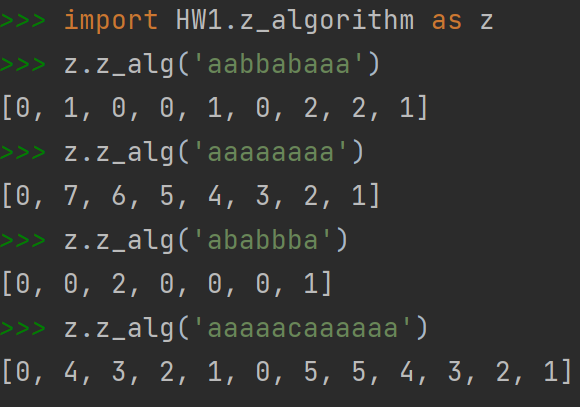
\includegraphics[]{example1.png}
    \caption{Examples using base z algorithm}
    \label{fig:z_alg}
\end{figure}

\begin{figure}[h]
    \centering
    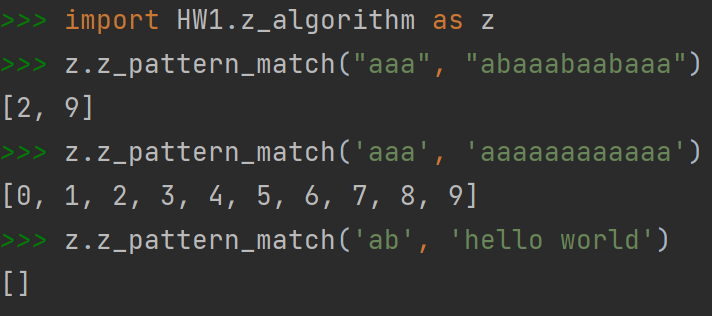
\includegraphics[]{example2.png}
    \caption{Examples using pattern matching}
    \label{fig:z_alg}
\end{figure}

I also did the bonus, which runs via the command line. Here is an example below showing functionality.

\end{document}